\section{Weak convergence of the centered NormFlowSDE inference scheme}
\label{app:diffusion}\label{sec:weak_conv_norm_flowsde}

This appendix gives the full argument behind the continuous-time interpretation in Section~\ref{sec:method}. The starting point is the trained, finite-step transition. We first construct an inference scheme that preserves that transition at its training interval, then prove convergence of its trajectories as the inference step decreases. The result concerns a conditional generative model; it does not identify its coefficients with the physical dynamics of the observed system.

\subsection{What is held fixed, and why the noise must be centered}

Write $h_0=\Delta t_{\mathrm{train}}>0$ for the physical interval of the trained transition and $h=\Delta t_{\mathrm{inf}}>0$ for the inference step. Fix a finite time horizon $[0,T]$ and a deterministic, continuous schedule $\xi=(u(\cdot),c(\cdot))$ of controls and observation features. The fitted parameters, training step $h_0$, and schedule $\xi$ remain fixed throughout; only the inference step $h$ tends to zero. Any step-size inputs to the networks are held at their training values. The initial state $z_0\in\R^d$ is supplied by the data and is also fixed. Every inference chain and the limiting process start from this same value, $Z_0^h=Z_0=z_0$. Conditioning on $z_0$ is implicit in all probabilities and expectations below. We retain the schedule in every coefficient, with
\begin{align*}
 f_\varphi(z,t;\xi)&:=f_\varphi(z,t,u(t),c(t)),\\
 g_\phi(\epsilon;z,t,\xi)&:=g_\phi(\epsilon;z,t,u(t),c(t)).
\end{align*}
The resulting coefficients must satisfy the stated assumptions for this fixed $\xi$; the constants below may depend on $\xi$. At each trained time $t_k$, $c(t_k)$ is the feature computed from the preceding observation window defined in Section~\ref{sec:method}. 

We use $z\in\R^d$ for a fixed state value and $Z$ for a random state. At time $t$, the trained update is
\begin{equation}\label{eq:trainingupdate}
 \begin{aligned}
 Z'&=z+h_0 f_\varphi(z,t;\xi)+\sqrt{h_0}\,g_\phi(\epsilon;z,t,\xi),\\
 \epsilon\mid z,t,\xi&\sim\N(0,I_d).
 \end{aligned}
\end{equation}
where $f_\varphi$ is the drift network and $g_\phi$ is the conditional flow. Assume its conditional mean exists, and define
\begin{align}\label{eq:centerednoise}
 m_\phi(z,t;\xi)&=\E_\epsilon[g_\phi(\epsilon;z,t,\xi)],\\
 \eta_c(z,t,\epsilon;\xi)&=g_\phi(\epsilon;z,t,\xi)-m_\phi(z,t;\xi).\notag
\end{align}
Here and below, $\E_\epsilon$ denotes integration over $\epsilon\sim\N(0,I_d)$ with the displayed state, time, and schedule fixed. Thus $\E_\epsilon[\eta_c(z,t,\epsilon;\xi)]=0$. The effective drift of the trained transition is its expected increment per unit time:
\begin{equation}\label{eq:effectivedrift}
 b_{\mathrm{eff}}(z,t;\xi)
 =f_\varphi(z,t;\xi)+\frac{m_\phi(z,t;\xi)}{\sqrt{h_0}}
 =\frac{\E[Z'-z\mid z,t,\xi]}{h_0}.
\end{equation}
Using this drift and the centered noise gives the inference map 
\begin{equation}\label{eq:refinement}
 F_{h,t}(z,\epsilon;\xi)
 =z+h b_{\mathrm{eff}}(z,t;\xi)+\sqrt h\,\eta_c(z,t,\epsilon;\xi).
\end{equation}
We distinguish the fixed training step $h_0$ from the inference step $h$ to preserve the learned transition at $h=h_0$. Centering the stochastic increment and compensating the drift then avoid a divergent mean contribution as $h\to0$.


\subsection{The limiting process and sufficient assumptions}\label{sec:limit-statement}

Repeated application of the inference map in Equation~\eqref{eq:refinement}, at times $t_k=kh$, gives
\begin{equation}\label{eq:centered}
 Z^h_{k+1}=Z^h_k+h b_{\mathrm{eff}}(Z^h_k,t_k;\xi)
                 +\sqrt h\,\eta_c(Z^h_k,t_k,\epsilon_k;\xi).
\end{equation}
For a current state $z$, the increment has conditional mean $h b_{\mathrm{eff}}(z,t;\xi)$ and covariance $hA(z,t;\xi)$, where
\begin{equation}\label{eq:limitcovariance}
 A(z,t;\xi)=\E_\epsilon[\eta_c(z,t,\epsilon;\xi)\eta_c(z,t,\epsilon;\xi)^\top].
\end{equation}
This identifies the candidate diffusion: its drift is $b_{\mathrm{eff}}$ and its diffusion covariance is $A$. Write its noise coefficient as a matrix $\sigma$ satisfying $\sigma\sigma^\top=A$. The conditions below ensure that matching these local moments also leads to convergence of complete trajectories.

\begin{assumption}[Conditions for diffusion convergence]\label{ass:limit}
On the finite horizon $[0,T]$, assume the following.
\begin{enumerate}
\item \textnormal{\bfseries Regular drift and diffusion.}\label{ass:limit-regularity}
The functions $b_{\mathrm{eff}}(z,t;\xi)$ and a covariance factor $\sigma(z,t;\xi)$ with $\sigma\sigma^\top=A$ are jointly continuous in $(z,t)$, globally Lipschitz in $z$, and of at most linear growth in $z$. The Lipschitz and growth constants are uniform in $t\in[0,T]$. These conditions control the trajectories and ensure uniqueness of the limiting SDE.
\item \textnormal{\bfseries Controlled noise moments.}\label{ass:limit-moments}
The centered noise $\eta_c$ is jointly measurable, and its third moment is bounded on every bounded state region, uniformly in time:
\begin{equation}\label{eq:local-third-assumption}
 \sup_{\norm z\leq R,\,t\in[0,T]}
 \E_\epsilon\norm{\eta_c(z,t,\epsilon;\xi)}^3<\infty,
 \qquad R<\infty.
\end{equation}
This condition controls the Taylor approximation error and the probability of large increments.
\item \textnormal{\bfseries Given initial state and independent noise.}\label{ass:limit-initial}
Every chain starts at the data-provided state $Z_0^h=z_0$. With $z_0$ and $\xi$ fixed, the Gaussian inputs $\epsilon_k\sim\N(0,I_d)$ are independent across steps. Thus trajectory randomness comes from the generated increments, not from sampling an initial state.
\end{enumerate}
\end{assumption}

\begin{theorem}[Weak convergence of the centered inference scheme]\label{thm:weak}
Under Assumption~\ref{ass:limit}, the paths generated by Equation~\eqref{eq:centered}, held constant between grid points as $\bar Z^h_t=Z^h_{\lfloor t/h\rfloor}$, satisfy
\[
 \operatorname{Law}(\bar Z^h\mid\xi)
 \Longrightarrow\operatorname{Law}(Z\mid\xi)
 \qquad(h\to0),
\]
in $D([0,T],\R^d)$ with the Skorokhod $J_1$ topology. The limit $Z$ is the unique-in-law solution of
\begin{equation}\label{eq:limit}
 \begin{aligned}
 dZ_t&=b_{\mathrm{eff}}(Z_t,t;\xi)\,dt+\sigma(Z_t,t;\xi)\,dW_t,\\
 Z_0&=z_0.
 \end{aligned}
\end{equation}
Conditional on the fixed data, $W$ is a standard $d$-dimensional Brownian motion. For every three-times continuously differentiable test function $v$ with compact support, the discrete generators also converge uniformly on bounded state regions and $t\in[0,T]$, as specified in Equation~\eqref{eq:generator} below.
\end{theorem}

The theorem compares distributions of whole trajectories. The space $D([0,T],\R^d)$ contains right-continuous paths with left limits, including the piecewise-constant paths $\bar Z^h$. Its Skorokhod $J_1$ topology allows small shifts in jump times when comparing paths \citep{skorokhod1956limit}; the limiting SDE paths are continuous. Section~\ref{sec:consistency-proof} now shows how the three assumptions turn the local moment match into this path-convergence result.

\subsection{Proof of Theorem~\ref{thm:weak}}\label{sec:consistency-proof}
The proof has two tasks: show that the trajectory distributions have limits, and identify those limits. Step~1 calculates the expected change over one inference step. Steps~2--4 then control whole trajectories: they prevent escape to arbitrarily large states, remove persistent jumps, and bound changes over short time intervals. Step~5 shows that any resulting limit must have the law of the SDE in Equation~\eqref{eq:limit}. We use the standard diffusion-approximation result of \citet{ethier1986markov,kushner2001numerical} to connect the path estimates and the limiting expected-change identity.

\paragraph{1. Identify the local diffusion limit.}
For a scalar test function $v\in C_c^3(\R^d)$, meaning that $v$ has three continuous derivatives and compact support, define
\begin{equation}\label{eq:discretegenerator}
 \mathcal L_{h,t}^{\xi}v(z)
 =\frac{\E_\epsilon[v(F_{h,t}(z,\epsilon;\xi))]-v(z)}h.
\end{equation}
This is the expected change of $v$ in one inference step, divided by the step duration. To calculate its limit, fix $(z,t,\xi)$ and write
$\Delta=h b_{\mathrm{eff}}(z,t;\xi)+\sqrt h\,\eta_c(z,t,\epsilon;\xi)$.
Throughout this local calculation, the arguments $(z,t,\xi)$ are held fixed and suppressed on $b_{\mathrm{eff}}$, $\eta_c$, and $A$:
\begin{align}\label{eq:proofmoments}
 \E[\Delta\mid z,t,\xi]
 &=h b_{\mathrm{eff}}+\sqrt h\,\E_\epsilon[\eta_c]
 =h b_{\mathrm{eff}},\notag\\
 \E[\Delta\Delta^\top\mid z,t,\xi]
 &=h^2b_{\mathrm{eff}}b_{\mathrm{eff}}^\top
   +h\E_\epsilon[\eta_c\eta_c^\top]+h^{3/2}\bigl(
 b_{\mathrm{eff}}\E_\epsilon[\eta_c]^\top
 +\E_\epsilon[\eta_c]b_{\mathrm{eff}}^\top\bigr)\notag\\
 &=h^2b_{\mathrm{eff}}b_{\mathrm{eff}}^\top+hA.
\end{align}
The $h^{3/2}$ line displays both drift--noise cross terms. They vanish because the noise is centered, $\E_\epsilon[\eta_c]=0$. The remaining noise term is its covariance $A$, defined in Equation~\eqref{eq:limitcovariance}.

Taylor's formula gives
\begin{equation}\label{eq:taylorexpansion}
 v(z+\Delta)-v(z)
 =\nabla v(z)^\top\Delta
  +\tfrac12\Delta^\top\nabla^2v(z)\Delta+R_v(z,\Delta),
 \qquad |R_v(z,\Delta)|\leq C_v\norm\Delta^3.
\end{equation}
Here $\nabla v$ and $\nabla^2v$ are the gradient and Hessian. To control the remainder, we need the \emph{third absolute moment of the full increment} $\Delta$. The drift is bounded on each region $\norm z\leq R$, $t\in[0,T]$, and the noise third moment is bounded by Equation~\eqref{eq:local-third-assumption}. Hence, for $0<h\leq1$,
\begin{align}\label{eq:thirdmoment}
 \E[\norm\Delta^3\mid z,t,\xi]
 &\leq4h^3\norm{b_{\mathrm{eff}}(z,t;\xi)}^3
   +4h^{3/2}\E_\epsilon\norm{\eta_c(z,t,\epsilon;\xi)}^3\notag\\
 &\leq C_{R,T}h^{3/2},
 \qquad \norm z\leq R,\quad t\in[0,T].
\end{align}
The constant is independent of $h$, $z$, and $t$ within this region. It is derived from, and distinct from, the assumed noise-moment bound.

Substituting the moments from Equation~\eqref{eq:proofmoments} into the expected Taylor expansion gives the full generator calculation:
\begin{align}\label{eq:generator-error}
 \mathcal L_{h,t}^{\xi}v(z)
 &=\frac1h\left(
 \nabla v(z)^\top\E_\epsilon\Delta
 +\frac12\operatorname{tr}\,\left(\nabla^2v(z)\E_\epsilon[\Delta\Delta^\top]\right)
 +\E_\epsilon R_v(z,\Delta)\right)\notag\\
 &=\frac1h\left(
 h\nabla v(z)^\top b_{\mathrm{eff}}
 +\frac12\operatorname{tr}\,\left(\nabla^2v(z)
       [hA+h^2b_{\mathrm{eff}}b_{\mathrm{eff}}^\top]\right)
 +\E_\epsilon R_v(z,\Delta)\right)\notag\\
 &=b_{\mathrm{eff}}^\top\nabla v(z)
   +\frac12\operatorname{tr}\,\left(A\nabla^2v(z)\right)
   +\frac h2 b_{\mathrm{eff}}^\top\nabla^2v(z)b_{\mathrm{eff}}
   +\frac{\E_\epsilon R_v(z,\Delta)}h .
\end{align}
The last two terms vanish uniformly on each bounded state region, since
\begin{align}\label{eq:generator-remainder}
 &\sup_{\norm z\leq R,\,t\in[0,T]}
 \left|\frac h2 b_{\mathrm{eff}}^\top\nabla^2v(z)b_{\mathrm{eff}}
       +\frac{\E_\epsilon R_v(z,\Delta)}h\right|\notag\\
 &\quad\leq
 \frac h2\sup_{\norm z\leq R,\,t\in[0,T]}
       \bigl(\norm{b_{\mathrm{eff}}}^2\norm{\nabla^2v(z)}_{\mathrm{op}}\bigr)
 +\frac{C_v}h\sup_{\norm z\leq R,\,t\in[0,T]}\E_\epsilon\norm\Delta^3
 \leq C_{R,T,v}(h+\sqrt h)\longrightarrow0.
\end{align}
Here $\norm{\cdot}_{\mathrm{op}}$ is the matrix operator norm. Thus the limiting generator is
\begin{equation}\label{eq:generator}
 \mathcal L_t^{\xi}v(z)
 =\lim_{h\to0}\mathcal L_{h,t}^{\xi}v(z)
 \overset{\mathrm{(\ref{eq:discretegenerator}),\,(\ref{eq:refinement})}}{=}
 \lim_{h\to0}\frac{
 \E_\epsilon[v(F_{h,t}(z,\epsilon;\xi))-v(z)]}{h}.
\end{equation}
Equations~\eqref{eq:generator-error}--\eqref{eq:generator-remainder} identify this limiting expected change with the drift and covariance terms of the candidate SDE. This proves the local conclusion of Theorem~\ref{thm:weak}; the remaining steps concern entire paths.

\paragraph{2. Bound the probability of leaving a large state region.}
The local calculation above is uniform only when the state stays in a bounded region. For a radius $R>\norm{z_0}$, we use the closed Euclidean ball centered at the origin,
\begin{equation}\label{eq:state-ball}
 \overline B(0,R):=\{z\in\R^d:\norm z\leq R\}.
\end{equation}
Here $\norm{\cdot}$ is the Euclidean norm, so the ball contains every state whose distance from the origin is at most $R$, including its boundary. We need to show that paths are unlikely to leave this ball over the entire time horizon, with a bound that does not deteriorate as $h$ decreases. We set $N_h=\lfloor T/h\rfloor$ and use the notation
\[
 b_k=b_{\mathrm{eff}}(Z_k^h,t_k;\xi),\qquad
 A_k=A(Z_k^h,t_k;\xi),\qquad
 \eta_k=\eta_c(Z_k^h,t_k,\epsilon_k;\xi).
\]
The linear-growth assumption gives
\begin{equation}\label{eq:innovation-growth}
 \norm{b_{\mathrm{eff}}(z,t;\xi)}^2+
 \E_\epsilon\norm{\eta_c(z,t,\epsilon;\xi)}^2
 =\norm{b_{\mathrm{eff}}(z,t;\xi)}^2+\operatorname{tr}A(z,t;\xi)
 \leq C(1+\norm z^2).
\end{equation}
We measure the size of a state by $V(z)=1+\norm z^2$. Centering and the growth bound imply, for $0<h\leq1$,
\begin{align}\label{eq:one-step-size}
 \E[V(Z_{k+1}^h)\mid Z^h_{0:k},\xi]
 &=1+\norm{Z_k^h+h b_k}^2+h\operatorname{tr}A_k\notag\\
 &\leq1+(1+h)\norm{Z_k^h}^2+(h+h^2)\norm{b_k}^2
          +h\operatorname{tr}A_k\notag\\
 &\leq(1+Ch)V(Z_k^h).
\end{align}
Here $Z^h_{0:k}$ denotes the generated history through step $k$. The bound says that the expected squared size grows by a factor at most $1+Ch$ per step.

To turn this into a bound for the whole path, we freeze a copy of the chain at its first exit from $\overline B(0,R)$. Exit from this closed ball means $\norm{Z_k^h}>R$:
\[
 \tau_R=\inf\{k\leq N_h:\norm{Z_k^h}>R\},\qquad
 Y_k^h=Z^h_{\min(k,\tau_R)},\qquad \inf\varnothing=\infty.
\]
This stopped copy is only a proof device; it does not change the inference algorithm. Before exit it follows the original chain, including the step that crosses the boundary. After exit it stays at that exit state. Equation~\eqref{eq:one-step-size} therefore also bounds its expected size, and iteration gives
\begin{align}\label{eq:stopped-size}
 \E[V(Y_{k+1}^h)\mid Z^h_{0:k},\xi]
 &\leq(1+Ch)V(Y_k^h),\notag\\
 \E[V(Y_{N_h}^h)\mid\xi]
 &\leq(1+Ch)^{N_h}V(z_0)
 \leq e^{CT}(1+\norm{z_0}^2)=:C_T.
\end{align}
If any state leaves the ball, the frozen final state has squared norm greater than $R^2$. Hence
\begin{equation}\label{eq:containment}
 \Pr\,\left(\max_{k\leq N_h}\norm{Z_k^h}>R\,\middle|\,\xi\right)
 =\Pr(\tau_R\leq N_h\mid\xi)
 \leq\frac{\E[V(Y_{N_h}^h)\mid\xi]}{1+R^2}
 \leq\frac{C_T}{1+R^2}.
\end{equation}
The same bound applies to $\sup_{t\leq T}\norm{\bar Z_t^h}$. For any probability tolerance $\varepsilon>0$, we can choose $R$ large enough that $C_T/(1+R^2)\leq\varepsilon$. This single radius works for every $0<h\leq1$: the process $\bar Z^h$ remains in $\overline B(0,R)$ throughout $[0,T]$ with probability at least $1-\varepsilon$. Because closed bounded balls in $\R^d$ are compact, this is the \emph{compact containment condition} of \citet[Chapter~3, Remark~7.3, p.~129]{ethier1986markov}.

\paragraph{3. Combine the one-step and whole-path jump bounds.}
Fix a jump threshold $a>0$. Equation~\eqref{eq:thirdmoment} bounds the third absolute moment of the full increment. Since $\norm\Delta^2\leq\norm\Delta^3/a$ whenever $\norm\Delta>a$,
\begin{equation}\label{eq:smalljumps}
 \sup_{\norm z\leq R,\,t\in[0,T]}
 \frac1h\E[\norm\Delta^2\boldsymbol 1_{\{\norm\Delta>a\}}\mid z,t,\xi]
 \qquad\leq\frac1{ah}
 \sup_{\norm z\leq R,\,t\in[0,T]}\E[\norm\Delta^3\mid z,t,\xi]
 \leq\frac{C_{R,T}}a\sqrt h\longrightarrow0.
\end{equation}
The indicator selects increments larger than $a$. This proves that large increments contribute vanishing second moment per unit time.

We also need the probability of encountering even one large jump along the path. The same third-moment estimate bounds each such probability by $C_{R,T}h^{3/2}/a^3$ while the starting state is inside the ball. There are at most $T/h$ increments. Adding these probabilities and the escape probability from Step~2 gives
\begin{align}\label{eq:maximum-jump}
 \Pr\,\left(\max_{k<N_h}\norm{Z_{k+1}^h-Z_k^h}>a\,\middle|\,\xi\right)
 &\quad\leq\Pr(\tau_R\leq N_h\mid\xi)
 +\sum_{k<N_h}\Pr\,\left(\norm{Z_{k+1}^h-Z_k^h}>a,\quad k<\tau_R\,\middle|\,\xi\right)\notag\\
 &\quad\leq\frac{C_T}{1+R^2}+\frac{T}{h}\frac{C_{R,T}h^{3/2}}{a^3}
 =\frac{C_T}{1+R^2}+\frac{T C_{R,T}}{a^3}\sqrt h .
\end{align}
First choose $R$ large, then let $h$ decrease. The largest jump over the whole horizon tends to zero in probability.

\paragraph{4. Bound the change over a short time interval.}
Small individual jumps do not rule out many small increments adding up rapidly. For example, continuous paths $x_n(t)=\sin(nt)$ stay bounded and have no jumps, yet change by order one over intervals of length $1/n$. 

Start at a grid index $K\leq N_h$ that may be chosen from the generated history, such as the first threshold crossing, capped at $N_h$. The choice cannot use future noise: whether $K\leq k$ must be determined at step $k$. Look ahead a fixed number $m$ of steps, ending at $L=\min(K+m,N_h)$; their duration is at most $\ell=mh$. We first bound the change of the stopped copy $Y^h$ from Step~2, so every active update starts inside the ball. Set
\[
 B_R=\sup_{\norm z\leq R,\,t\in[0,T]}\norm{b_{\mathrm{eff}}(z,t;\xi)},
 \qquad
 D_R=\sup_{\norm z\leq R,\,t\in[0,T]}\operatorname{tr}A(z,t;\xi).
\]
Both constants are finite. Let $I_j$ equal one when $K\leq j<L$ and $j<\tau_R$, and zero otherwise. There are at most $m$ active steps, so $\sum_j I_j\leq m$. The increment splits into accumulated drift and noise:
\begin{equation}\label{eq:interval-decomposition}
 Y_L^h-Y_K^h
 =\underbrace{\sum_{j<N_h}I_j h b_j}_{D_{K,m}^h}
  +\underbrace{\sum_{j<N_h}I_j\sqrt h\,\eta_j}_{M_{K,m}^h}.
\end{equation}
Each $I_j$ is determined before $\epsilon_j$ is drawn. Thus the active noise increments still have zero conditional mean, and cross terms between different noise increments vanish. Consequently,
\begin{align}\label{eq:interval-components}
 \norm{D_{K,m}^h}^2
 &\leq\left(\sum_{j<N_h}I_jh B_R\right)^2
 \leq B_R^2\ell^2,\notag\\
 \E[\norm{M_{K,m}^h}^2\mid\xi]
 &=\E\,\left[\sum_{j<N_h}I_jh\operatorname{tr}A_j\,\middle|\,\xi\right]
 \leq D_R\ell.
\end{align}
The drift grows with elapsed time; the noise \emph{variance} grows with elapsed time. We do not assume that the accumulated drift and noise are independent. Using $\norm{D+M}^2\leq2\norm D^2+2\norm M^2$ gives
\begin{equation}\label{eq:short-increment}
 \E[\norm{Y_L^h-Y_K^h}^2\mid\xi]
 \leq2B_R^2\ell^2+2D_R\ell.
\end{equation}
Except when the original path exits the ball, its increment equals that of the stopped copy. For $\ell\leq\delta+h$,
\begin{align}\label{eq:short-increment-probability}
 \Pr(\norm{Z_L^h-Z_K^h}>a\mid\xi)
 &\leq\Pr(\tau_R\leq N_h\mid\xi)
    +\frac{\E[\norm{Y_L^h-Y_K^h}^2\mid\xi]}{a^2}\notag\\
 &\leq\frac{C_T}{1+R^2}
   +\frac{2}{a^2}\left[B_R^2(\delta+h)^2+D_R(\delta+h)\right].
\end{align}
Choose $R$ large first. With that radius fixed, the second term tends to zero as the interval length $\delta$ and step $h$ decrease. Thus a large change is unlikely over a short interval, even when its starting time is selected from the generated history.

For starting times between grid points, rounding to the grid alters the compared increment by at most two grid jumps; Step~3 shows that this error vanishes. The containment and short-interval estimates are the compactness conditions in the cited diffusion-approximation result: every sequence $h\to0$ has a subsequence whose path laws converge. This property is called \emph{tightness}. Together with the vanishing jumps, these bounds ensure that the possible limits have continuous paths.

\paragraph{5. Identify the limit through its expected changes.}
Steps~2--4 establish the existence of subsequential limits, but do not yet specify their law. Let $X$ denote any such limit. We now show why its law must be that of the SDE in Equation~\eqref{eq:limit}.

\emph{From one step to an interval.}
The generator predicts the expected change of any smooth test function $v$:
\begin{equation}\label{eq:conditional-test-increment}
 \E[v(Z^h_{j+1})-v(Z^h_j)-h\mathcal L_{h,t_j}^{\xi}v(Z_j^h)
       \mid Z^h_{0:j},\xi]=0.
\end{equation}
Thus \emph{actual change minus predicted change} has zero conditional mean. For grid indices $p<q$, sum these differences for the stopped copy from Step~2. The state changes telescope, giving
\begin{equation}\label{eq:stopped-expected-change}
 \E\,\left[
 \underbrace{v(Y_q^h)-v(Y_p^h)}_{\mbox{\scriptsize actual change}}
 -\underbrace{\sum_{j=p}^{q-1}\boldsymbol 1_{\{j<\tau_R\}}
       h\mathcal L_{h,t_j}^{\xi}v(Z_j^h)}_{\mbox{\scriptsize accumulated predicted change}}
 \,\middle|\,Z^h_{0:p},\xi\right]=0.
\end{equation}
Stopping ensures that every rate in this sum is evaluated inside the region where Step~1 gives uniform convergence.

\emph{From the discrete sum to a time integral.}
Replacing each discrete rate by $\mathcal L_{t_j}^{\xi}v$ incurs a total error bounded by
\[
 \left|\sum_{j=p}^{q-1}\boldsymbol 1_{\{j<\tau_R\}}h
  \bigl(\mathcal L_{h,t_j}^{\xi}v-\mathcal L_{t_j}^{\xi}v\bigr)(Z_j^h)\right|
 \leq T\sup_{\norm z\leq R,\,t\in[0,T]}
       |\mathcal L_{h,t}^{\xi}v(z)-\mathcal L_t^{\xi}v(z)|
 \longrightarrow0.
\]
Continuity of the limiting paths and coefficients turns the sum of limiting rates into its time integral. The cited diffusion-approximation result passes the stopped conditional-mean identity to the limit. Step~2 then allows $R$ to increase without retaining a stopped boundary. For $0\leq s\leq t\leq T$, the resulting identity is
\begin{equation}\label{eq:limit-expected-change}
 \E\,\left[
 \underbrace{v(X_t)-v(X_s)}_{\mbox{\scriptsize actual change}}
 -\underbrace{\int_s^t\mathcal L_r^\xi v(X_r)\,dr}_{\mbox{\scriptsize accumulated predicted change}}
 \,\middle|\,X_{[0,s]},\xi\right]=0,
 \qquad X_0=z_0.
\end{equation}
Here $X_{[0,s]}$ is the path observed up to time $s$. Both $v$ and $\mathcal L_t^\xi v$ are bounded because $v$ has compact support, so the limiting identity is valid over the full horizon.

\emph{Why this identifies the SDE.}
For the candidate SDE solution $Z$, It\^o's formula gives exactly the same rule:
\begin{align}\label{eq:ito-expected-change}
 v(Z_t)-v(Z_s)-\int_s^t\mathcal L_r^\xi v(Z_r)\,dr
 &=\int_s^t\nabla v(Z_r)^\top\sigma(Z_r,r;\xi)\,dW_r,\notag\\
 \E\,\left[\int_s^t\nabla v(Z_r)^\top\sigma(Z_r,r;\xi)\,dW_r
       \,\middle|\,Z_{[0,s]},\xi\right]&=0.
\end{align}
The stochastic integral represents the unpredicted fluctuation; its conditional mean is zero. Requiring this expected-change rule for \emph{every} $v\in C_c^3$, together with continuous paths and $X_0=z_0$, is the standard characterization of the diffusion law used in the cited result. The regularity assumption guarantees that this law is unique. Hence
\[
 \mbox{any subsequential limit }X
 \quad\Longrightarrow\quad
 \operatorname{Law}(X\mid\xi)=\operatorname{Law}(Z\mid\xi).
\]
Every possible subsequential limit is therefore the same SDE law, so the entire family of path laws converges. This completes the proof of Theorem~\ref{thm:weak}.\hfill$\square$

\subsection{Accuracy of approximate centering}

The theorem uses the exact noise mean $m_\phi$. If it is replaced by an approximation $\widehat m_h$, the approximation affects both the drift compensation and the centered noise. The following result states how accurate it must be as the inference step decreases.

\begin{corollary}[Approximate conditional means]\label{cor:centering}
Suppose Assumption~\ref{ass:limit} holds. Replace $m_\phi$ by a deterministic measurable approximation $\widehat m_h$ in both the compensated drift and centered noise. If
\begin{equation}\label{eq:centererror}
 \sup_{z,\,t\in[0,T]}\norm{\widehat m_h(z,t;\xi)-m_\phi(z,t;\xi)}=o(\sqrt h),
\end{equation}
then the same diffusion limit holds.
\end{corollary}
\paragraph{Proof.}
Let $e_h(z,t;\xi)=\widehat m_h(z,t;\xi)-m_\phi(z,t;\xi)$ be the mean-estimation error. The drift increment gains $h e_h/\sqrt{h_0}$, while the noise increment loses $\sqrt h\,e_h$. Substituting the approximate mean and collecting these two changes gives
\begin{align}\label{eq:approximateupdate}
 \widehat Z'
 &=z+h\left(f_\varphi(z,t;\xi)+\frac{\widehat m_h(z,t;\xi)}{\sqrt{h_0}}\right)+\sqrt h\left(g_\phi(\epsilon;z,t,\xi)-\widehat m_h(z,t;\xi)\right)\notag\\
 &=F_{h,t}(z,\epsilon;\xi)
   +\left(\frac h{\sqrt{h_0}}-\sqrt h\right)e_h(z,t;\xi).
\end{align}
The last line separates the exact inference update from the error caused by approximate centering. For a continuous-time limit, the relevant error is the added drift \emph{per unit time}, obtained by dividing the extra term by $h$:
\begin{equation}\label{eq:centering-drift-error}
 \frac{\widehat Z'-F_{h,t}(z,\epsilon;\xi)}h
 =\left(\frac1{\sqrt{h_0}}-\frac1{\sqrt h}\right)e_h(z,t;\xi).
\end{equation}
Its norm is uniformly bounded by
\[
 \left(\frac1{\sqrt{h_0}}+\frac1{\sqrt h}\right)
 \sup_{z,\,t\in[0,T]}\norm{e_h(z,t;\xi)}\longrightarrow0
\]
under Equation~\eqref{eq:centererror}. Thus the added drift vanishes uniformly, while the centered random part remains unchanged. This bounded perturbation preserves the moment and path bounds in Steps~1--4, and the limiting expected-change rule in Step~5 is unchanged. The same diffusion limit follows.\hfill$\square$

At $h=h_0$, the error coefficient in Equation~\eqref{eq:approximateupdate} is zero: using the same mean estimate in the drift and noise preserves the trained update exactly. As $h\to0$, however, a fixed nonzero estimation error is amplified by the $1/\sqrt h$ factor in Equation~\eqref{eq:centering-drift-error}. 

\subsection{Scope of the convergence result}\label{sec:limit-scope}

Theorem~\ref{thm:weak} establishes convergence of conditional trajectory distributions for the centered inference scheme under the stated assumptions. Only the first two conditional moments remain in the limit, so non-Gaussian finite-step increments can approach an It\^o diffusion. The following distinctions specify what this result does and does not provide.

\paragraph{Weak convergence and individual paths.}
The theorem concerns distributions of paths. It does not compare an individual simulated path with an SDE path driven by the same Brownian realization, or prove that their samplewise error tends to zero. Such a strong-convergence statement requires a specified coupling and a separate error analysis.

\paragraph{The training step and smaller inference steps.}
The construction preserves one trained transition at $h=h_0$. This does not imply that several smaller steps reproduce that transition, or that the limiting SDE has the same transition law over an interval of length $h_0$. Convergence as $h\to0$ is distinct from equality of finite-interval distributions.

\paragraph{Numerical accuracy and learned models.}
The theorem gives no convergence rate or adaptive-step guarantee. Its regularity and moment assumptions must be checked for the learned coefficients. Finite-step sampling and density evaluation in Section~\ref{sec:method} remain valid without the optional centering used for this continuous-time argument.

\paragraph{Numerical illustration.}
Figure~\ref{fig:weak-convergence-ou} applies the centered inference scheme to a trained NormFlowSDE transition whose data-generating process is a standard SDE with a known solution. The trained update is held fixed, as in Theorem~\ref{thm:weak}, and only the inference step $h$ is reduced.

\begin{figure}[t]
\centering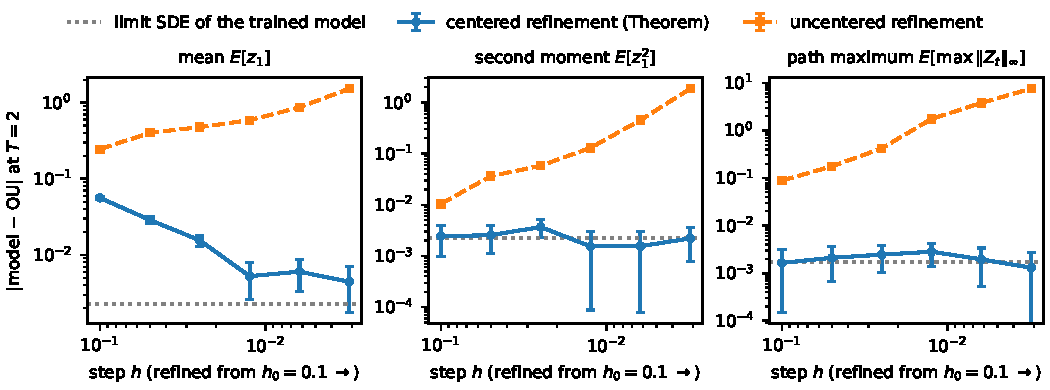
\includegraphics[width=\linewidth]{figures/weak_convergence_ou_row_print.pdf}
\caption{Centered refinement of a trained NormFlowSDE transition recovers a standard SDE. The reference process is the two-dimensional Ornstein--Uhlenbeck SDE $dZ=-KZ\,dt+S\,dW$ with $K=[1,\,0.8;\,-0.8,\,1]$, $S=[0.6,\,0;\,0.3,\,0.4]$ (rows separated by semicolons) and $Z_0=(2,-1)$. A NormFlowSDE model (drift network and conditional RealNVP noise flow, $\alpha=1.5$) was fitted by its exact one-step likelihood to transitions $z'=z-h_0Kz+\sqrt{h_0}\,S\eta$ at $h_0=0.1$, where $\eta$ has independent, skewed two-component-mixture coordinates with zero mean, unit variance and skewness $-0.38$. The finite-step increments are therefore non-Gaussian, while the only diffusion with the same first two moments is the reference process. With the fitted networks fixed, each panel shows the absolute error at $T=2$, relative to the exact Ornstein--Uhlenbeck law, of the mean of $z_1$, the second moment $z_1^2$, and the path maximum $\max_t\norm{Z_t}_\infty$ on the grid $t\in h_0\mathbb{N}$. The step decreases from $h_0$ to $h_0/32$ from left to right. Blue: the centered scheme of Theorem~\ref{thm:weak}, with $m_\phi$ and $A$ computed by $24\times24$ Gauss--Hermite quadrature. Orange: the uncentered refinement $z+hf_\varphi+\sqrt h\,g_\phi$. Dotted: the limit SDE of the fitted model, simulated by Euler--Maruyama at $h_0/128$; its distance to the reference process is the learning error that remains as $h\to0$. The fitted drift $b_{\rm eff}$ and diffusion $A$ differ from $-Kz$ and $SS^\top$ by at most $0.027$ and $0.0045$ on $[-2,2]^2$. The centered error of the mean decreases from $0.056$ at $h_0$, the bias of the coarse training chain, towards this learning-error floor; the other statistics are already near the floor at $h_0$. The fitted noise flow has a nonzero mean ($\norm{m_\phi}$ up to $0.83$), which is not identifiable from the drift in the trained update; without centering it acts as a drift of order $1/\sqrt h$, and the uncentered errors grow as $h$ decreases.}
\label{fig:weak-convergence-ou}
\end{figure}
